% Rozwinięcie AM II-02, AM II-03 i AM II-08.
\chapter{Szeregi funkcyjne}
\label{ma2:ch:function-series}

Niech $X$ będzie niepustym zbiorem, a $E$ przestrzenią
unormowaną nad $\K$. Wykorzystamy teorię szeregów
wektorowych z rozdziału \ref{ma2:ch:banach-series}
oraz zbieżności jednostajnej z rozdziału
\ref{ma2:ch:uniform-convergence}. Zupełność $E$
będziemy zakładać tam, gdzie jest potrzebna
do istnienia sumy szeregu.

\section{Sumy częściowe i kryterium Cauchy'ego}

\begin{definicja}
\label{ma2:def:function-series}
Dla ciągu funkcji $u_n:X\to E$, $n\ge1$, określamy
sumy częściowe $S_0(x)=0$ oraz
$S_N(x)=\sum_{n=1}^N u_n(x)$.
Szereg funkcyjny $\sum_{n\ge1}u_n$ nazywamy
zbieżnym punktowo (odpowiednio jednostajnie)
do $S:X\to E$, jeżeli ciąg $(S_N)$ jest zbieżny
punktowo (odpowiednio jednostajnie) do $S$.
Szereg nazywamy punktowo bezwzględnie zbieżnym,
jeżeli dla każdego $x\in X$ szereg liczbowy
$\sum_{n\ge1}\|u_n(x)\|$ jest zbieżny.
\end{definicja}
W przypadku pustej dziedziny wszystkie warunki
zbieżności zachodzą automatycznie.
Zbieżność punktowa oznacza dokładnie zbieżność
każdego szeregu wektorowego $\sum_n u_n(x)$.
Jednoznaczność sumy wynika z jednoznaczności
granicy punktowej. W dalszym ciągu szeregi
indeksowane od $0$ rozumiemy analogicznie.

\begin{twierdzenie}[Jednostajne kryterium Cauchy'ego]
\label{ma2:thm:function-series-cauchy}
Niech $u_n:X\to E$ dla $n\ge1$.
Jeśli szereg $\sum_n u_n$ jest jednostajnie zbieżny,
to
\[
 \forall\varepsilon>0\ \exists N\ge1\
 \forall q\ge p\ge N\ \forall x\in X:
 \quad \left\|\sum_{n=p}^q u_n(x)\right\|<\varepsilon.
\]
Jeżeli $E$ jest przestrzenią Banacha, warunek jest
również wystarczający. Jest wystarczający także
w niezupełnej przestrzeni $E$, jeśli szereg ma już
sumę punktową w $E$.
\end{twierdzenie}
\begin{proof}
Dla $q\ge p\ge1$ zachodzi
$\sum_{n=p}^q u_n=S_q-S_{p-1}$.
Jeżeli $(S_n)$ spełnia jednostajny warunek
Cauchy'ego z progiem $M$, to wybieramy $N=M+1$.
Odwrotnie, dla $m>n\ge N$ stosujemy warunek
z tezy z $p=n+1$, $q=m$. Dla $n>m$ korzystamy
z symetrii normy różnicy, a dla $n=m$ różnica
wynosi zero. Otrzymujemy jednostajny warunek
Cauchy'ego dla $(S_n)$.
Wszystkie wnioski wynikają teraz z twierdzenia
\ref{ma2:thm:uniform-cauchy} oraz uwagi o istniejącej
granicy punktowej po jego dowodzie.
\end{proof}

\begin{wniosek}
\label{ma2:cor:uniform-series-term}
Jednostajna zbieżność szeregu implikuje
jednostajną zbieżność jego wyrazów do zera.
\end{wniosek}
\begin{proof}
W kryterium \ref{ma2:thm:function-series-cauchy}
bierzemy $q=p=n$. Otrzymujemy warunek
jednostajnej zbieżności $(u_n)$ do zera.
\end{proof}
Warunek nie jest wystarczający: na dowolnym
niepustym $X$ funkcje $u_n(x)=1/n$ zbiegają
jednostajnie do zera, ale ich szereg jest
rozbieżny (AM I, rozdział 09, przykład szeregu
harmonicznego, etykieta \texttt{ma1:ex:harmonic-series}).

Jeżeli $X$ jest przestrzenią topologiczną,
wszystkie $u_n$ są ciągłe i szereg zbiega
jednostajnie, to suma $S$ jest ciągła:
każda suma częściowa jest ciągła, a twierdzenie
\ref{ma2:thm:uniform-continuous-limit} daje tezę.
Jeżeli $X$ jest metryczna, wystarcza również
zbieżność jednostajna na zbiorach zwartych
(twierdzenie \ref{ma2:thm:compact-uniform-continuity}).

\section{Kryterium Weierstrassa i zbieżność normalna}

\begin{definicja}
\label{ma2:def:normal-series}
Szereg $\sum_n u_n$ jest zbieżny normalnie na $X$,
jeśli dla każdego $n$ istnieje skończona liczba
$M_n=\sup_{x\in X}\|u_n(x)\|$ i
\[
 \sum_{n=1}^{\infty}M_n<\infty.
\]
Dla przestrzeni topologicznej $X$ mówimy o zbieżności
normalnej na zbiorach zwartych, jeśli warunek
zachodzi po ograniczeniu do każdego zwartego
$K\subseteq X$. Dla $K=\varnothing$ przyjmujemy
wszystkie normy supremum równe zero.
\end{definicja}

\begin{twierdzenie}[Kryterium Weierstrassa]
\label{ma2:thm:weierstrass-test}
Niech $E$ będzie przestrzenią Banacha. Jeśli
istnieje zbieżny szereg nieujemnych liczb
$\sum_n a_n$ taki, że
$\|u_n(x)\|\le a_n$ dla wszystkich $n,x$,
to szereg $\sum_n u_n$ jest zbieżny normalnie
i jednostajnie, a szereg funkcji
$\sum_n\|u_n(\cdot)\|$ jest jednostajnie zbieżny.
Dla sumy $S$ i każdego $N\ge0$ zachodzi
\[
 \sup_{x\in X}\|S(x)-S_N(x)\|
 \le\sum_{n>N}a_n.
\]
\end{twierdzenie}
\begin{proof}
Z definicji supremum mamy $0\le M_n\le a_n$.
Z porównania szeregów nieujemnych (AM I,
rozdział 09, etykieta \texttt{ma1:thm:series-comparison})
wynika $\sum_n M_n\le\sum_n a_n<\infty$.
Każde $u_n$ jest więc elementem przestrzeni $B(X,E)$,
która jest przestrzenią Banacha na mocy
twierdzenia \ref{ma2:thm:bounded}. Zastosowanie
twierdzenia \ref{ma2:thm:absolute-series} w tej
przestrzeni daje zbieżność w normie supremum
i oszacowanie reszty przez $\sum_{n>N}M_n$.
Z twierdzenia \ref{ma2:thm:uniform-criteria}
jest to zbieżność jednostajna.
Analogicznie, w przestrzeni Banacha $B(X,\R)$,
funkcje $v_n(x)=\|u_n(x)\|$ mają normy $M_n$,
więc ich szereg jest jednostajnie zbieżny.
\end{proof}
Nie jest konieczne, aby oszacowanie
$\|u_n(x)\|\le a_n$ zachodziło dla skończonego
początku szeregu: dla zbieżności jednostajnej
wystarczy oszacowanie ogona. Wtedy stosujemy
twierdzenie do ogona, a następnie dodajemy
skończoną sumę funkcji początkowych, która
nie zależy od indeksu sumy częściowej.
Jeśli choć jedna z tych początkowych funkcji
jest nieograniczona, cały szereg nie jest zbieżny
normalnie w sensie przyjętej definicji.
Na przykład dla $X=\R$, $E=\R$, $u_1(x)=x$
i $u_n(x)=0$ dla $n\ge2$, sumy częściowe
od indeksu $1$ są identyczne, ale
$\sup_{x\in\R}|u_1(x)|=+\infty$.
Dla niezupełnej przestrzeni $E$ oszacowanie
Weierstrassa wciąż daje jednostajny warunek
Cauchy'ego i zbieżność szeregu norm. Jeżeli
istnieje suma punktowa w $E$, daje także
zbieżność jednostajną i to samo oszacowanie reszty:
stosujemy nierówność trójkąta do skończonych
ogonów i przechodzimy do granicy przy ustalonym $x$,
po czym bierzemy supremum.

\begin{przyklad}[Szereg geometryczny]
\label{ma2:ex:function-geometric}
Dla $0\le r<1$ szereg $\sum_{n=0}^\infty z^n$
jest zbieżny normalnie na $\{z\in\C:|z|\le r\}$,
ponieważ $\sup_{|z|\le r}|z^n|=r^n$ (przy $r^0=1$).
Z twierdzenia o szeregu geometrycznym
(AM I, rozdział 09, etykieta \texttt{ma1:thm:geometric-series})
suma jest równa $1/(1-z)$. Błąd po wyrazie
o indeksie $N$ jest nie większy niż
$r^{N+1}/(1-r)$.
Każdy niepusty zwarty podzbiór otwartego koła
jednostkowego mieści się w kole o promieniu $r<1$,
bo ciągła funkcja $z\mapsto |z|$ osiąga na nim maksimum.
Stąd zbieżność normalna na zbiorach zwartych.
Na całym otwartym kole zbieżność nie jest jednostajna:
dla każdego $n\ge1$ supremum $|z|^n$ wynosi $1$,
co przeczy wnioskowi \ref{ma2:cor:uniform-series-term}.
\end{przyklad}

\section{Różne rodzaje zbieżności szeregów}

Z kryterium Weierstrassa w przestrzeni Banacha
wynika ciąg implikacji:
zbieżność normalna implikuje jednostajną
zbieżność szeregu norm, a ta implikuje
zbieżność jednostajną szeregu wektorowego.
Istotnie, jednostajny warunek Cauchy'ego dla
szeregu norm i nierówność
$\|\sum_{n=p}^q u_n(x)\|\le\sum_{n=p}^q\|u_n(x)\|$
dają warunek z twierdzenia
\ref{ma2:thm:function-series-cauchy}.
Zbieżność szeregu norm jednostajnie implikuje
też jego zbieżność punktową.
Poniższe przykłady pokazują, że własności te
nie są równoważne. W szczególności zbieżność
jednostajna i punktowa zbieżność bezwzględna
nie implikują jedna drugiej. Dla szeregu o wartościach
w przestrzeni niezupełnej zbieżność normalna
zapewnia jednostajny warunek Cauchy'ego, lecz
istnienie sumy wymaga dodatkowego założenia
(por. przykład \ref{ma2:ex:incomplete-series}
przeniesiony na funkcje stałe).

\begin{przyklad}[Jednostajna zbieżność bez zbieżności normalnej]
\label{ma2:ex:uniform-nonnormal}
Na $[0,1]$ niech $u_n(x)=(-1)^{n-1}/n$.
Szereg jest jednostajnie zbieżny, ponieważ
każda suma częściowa jest funkcją stałą,
a szereg liczbowy jest zbieżny z twierdzenia
\ref{ma1:thm:leibniz-series}.
Nie jest punktowo bezwzględnie zbieżny,
gdyż szereg modułów to szereg harmoniczny.
\end{przyklad}

\begin{przyklad}[Jednostajna zbieżność szeregu norm bez zbieżności normalnej]
\label{ma2:ex:absolute-uniform-nonnormal}
Dla $n\ge1$ niech
$I_n=[2^{-n},2^{1-n}]$,
$c_n=3\cdot2^{-n-1}$ i $h_n=2^{-n-1}$.
Na $[0,1]$ określamy
\[
 u_n(x)=\frac1n\max\{1-|x-c_n|/h_n,0\}.
\]
Funkcja $u_n$ jest ciągła i nieujemna, znika poza
wnętrzem $I_n$, a $u_n(c_n)=1/n$.
Wnętrza przedziałów $I_n$ są parami rozłączne.
W każdym punkcie co najwyżej jeden wyraz jest
niezerowy, więc od pewnego indeksu ciąg sum
częściowych w tym punkcie jest stały i suma
punktowa $S$ istnieje.
Dla $N\ge0$ mamy
\[
 \sup_{x\in[0,1]}|S(x)-S_N(x)|=\frac1{N+1}.
\]
Nierówność górna wynika z tego, że jedyny możliwy
niezerowy wyraz ogona ma indeks $n>N$,
a równość otrzymujemy dla $x=c_{N+1}$.
Zatem szereg norm (tu równy szeregowi funkcji)
jest jednostajnie zbieżny, lecz
$\sum_n\|u_n\|_\infty=\sum_n1/n=+\infty$.
\end{przyklad}

\begin{figure}[htbp]
\centering
\begin{tikzpicture}[x=11cm,y=3cm,>=Stealth]
 \draw[->] (0,0)--(1.04,0) node[right]{$x$};
 \draw[->] (0,0)--(0,1.13) node[above]{$y$};
 \foreach \n in {1,...,5}{
  \pgfmathsetmacro{\aa}{pow(2,-\n)}
  \pgfmathsetmacro{\bb}{2*\aa}
  \pgfmathsetmacro{\cc}{1.5*\aa}
  \pgfmathsetmacro{\hh}{1/\n}
  \draw[blue!70!black,thick,fill=blue!10]
       (\aa,0)--(\cc,\hh)--(\bb,0)--cycle;
  \node[above,font=\scriptsize] at (\cc,\hh) {$1/\n$};
 }
 \foreach \xx/\lab in {.25/{1/4},.5/{1/2},1/1}{
  \draw (\xx,0)--(\xx,-.025) node[below] {$\lab$};
 }
 \node[below left] at (0,0) {$0$};
\end{tikzpicture}
\caption{Rozłączne wnętrza przedziałów z przykładu
\ref{ma2:ex:absolute-uniform-nonnormal}.
Supremum ogona wynosi $1/(N+1)$, chociaż suma
supremów wyrazów jest nieskończona. Pokazano pięć
pierwszych funkcji.}
\label{ma2:fig:normal-hats}
\end{figure}
\FloatBarrier

\begin{przyklad}[Punktowa zbieżność bezwzględna bez jednostajnej]
\label{ma2:ex:pointwise-absolute-not-uniform}
Na $[0,1]$ połóżmy $u_n(x)=(1-x)x^n$ dla $n\ge1$.
Wyrazy są nieujemne i
$S_N(x)=x-x^{N+1}$ na mocy teleskopowania.
Dla $0\le x<1$ granica wynosi $x$, dla $x=1$
wynosi $0$. Zatem szereg jest punktowo bezwzględnie
zbieżny, ale $\sup_{[0,1]}|S-S_N|=1$:
dla $x<1$ różnica wynosi $x^{N+1}$, a w punkcie
$1$ wynosi zero. Zbieżność nie jest jednostajna.
\end{przyklad}

\paragraph{Rysunek 3D: sumy częściowe szeregu.}
Krzywe przedstawiają sumy częściowe $S_N(x)=x-x^{N+1}$.
Dla każdego $N$ wartość w $x=1$ wynosi zero;
przekroje uwidaczniają brak zbieżności jednostajnej.
Poniższy kod wymaga bibliotek NumPy i Plotly. Zapisuje samodzielny
plik HTML, w którym można obracać i powiększać wykres.
Rysunek \ref{ma2:fig:partial-sums-3d} przedstawia te same
krzywe; dla czytelności używamy na osi indeksu współrzędnej
$\log_2N$. Indeksy nadal są dyskretne.

\begin{figure}[htbp]
\centering
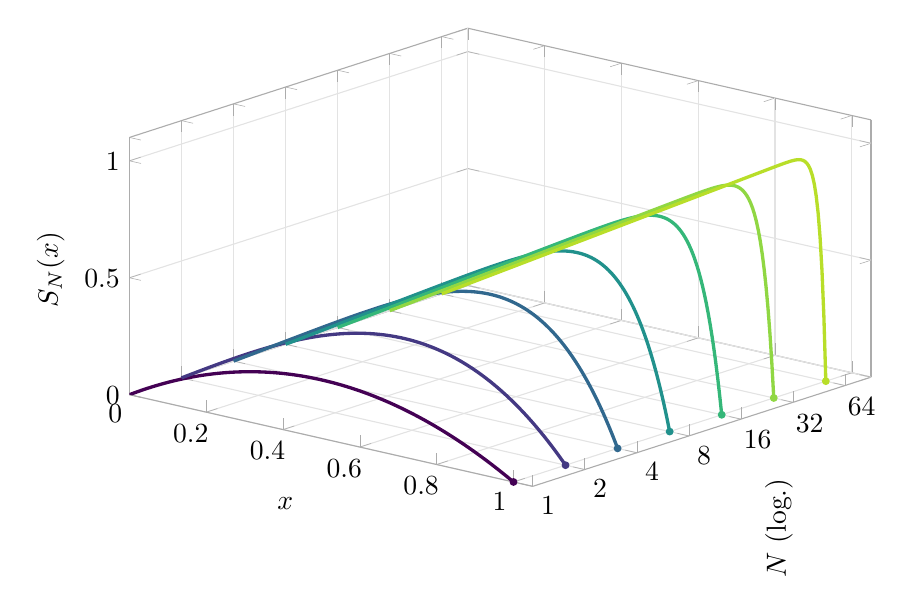
\begin{tikzpicture}
\definecolor{curve0}{HTML}{440154}
\definecolor{curve1}{HTML}{443983}
\definecolor{curve2}{HTML}{31688E}
\definecolor{curve3}{HTML}{21918C}
\definecolor{curve4}{HTML}{35B779}
\definecolor{curve5}{HTML}{90D743}
\definecolor{curve6}{HTML}{B8DE29}
\begin{axis}[width=11cm,height=7.4cm,view={40}{29},axis lines=box,grid=major,major grid style={draw=gray!22},axis line style={gray!65},tick style={gray!65},xmin=0,xmax=1.05,ymin=0,ymax=6.5,zmin=0,zmax=1.1,xlabel=$x$,ylabel={$N$ (log.)},zlabel={$S_N(x)$},ytick={0,1,2,3,4,5,6},yticklabels={1,2,4,8,16,32,64}]
\addplot3[very thick,curve0,domain=0:1,samples=201,samples y=1] (x,0,{x-x^(2)});
\addplot3[only marks,mark=*,mark size=1.2pt,curve0] coordinates {(1,0,0)};
\addplot3[very thick,curve1,domain=0:1,samples=201,samples y=1] (x,1,{x-x^(3)});
\addplot3[only marks,mark=*,mark size=1.2pt,curve1] coordinates {(1,1,0)};
\addplot3[very thick,curve2,domain=0:1,samples=201,samples y=1] (x,2,{x-x^(5)});
\addplot3[only marks,mark=*,mark size=1.2pt,curve2] coordinates {(1,2,0)};
\addplot3[very thick,curve3,domain=0:1,samples=201,samples y=1] (x,3,{x-x^(9)});
\addplot3[only marks,mark=*,mark size=1.2pt,curve3] coordinates {(1,3,0)};
\addplot3[very thick,curve4,domain=0:1,samples=201,samples y=1] (x,4,{x-x^(17)});
\addplot3[only marks,mark=*,mark size=1.2pt,curve4] coordinates {(1,4,0)};
\addplot3[very thick,curve5,domain=0:1,samples=201,samples y=1] (x,5,{x-x^(33)});
\addplot3[only marks,mark=*,mark size=1.2pt,curve5] coordinates {(1,5,0)};
\addplot3[very thick,curve6,domain=0:1,samples=201,samples y=1] (x,6,{x-x^(65)});
\addplot3[only marks,mark=*,mark size=1.2pt,curve6] coordinates {(1,6,0)};
\end{axis}
\end{tikzpicture}
\caption{Sumy częściowe $S_N(x)=x-x^{N+1}$ dla $N=1,2,4,8,16,32,64$. Oś indeksu ma skalę logarytmiczną, a każda krzywa kończy się w punkcie o wartości $S_N(1)=0$.}
\label{ma2:fig:partial-sums-3d}
\end{figure}

\begin{lstlisting}[language=Python]
import numpy as np
import plotly.graph_objects as go

x = np.linspace(0, 1, 501)
fig = go.Figure()
for n in [1, 2, 4, 8, 16, 32, 64]:
    fig.add_trace(go.Scatter3d(
        x=x, y=np.full_like(x, n), z=x-x**(n+1),
        mode="lines", name=f"N={n}"))
fig.update_layout(scene=dict(
    xaxis_title="x", yaxis_title="N", zaxis_title="S_N(x)"))
axis_style = dict(showbackground=True,
    backgroundcolor="#f5f6f7", gridcolor="#d5dbe0",
    zerolinecolor="#b0b8bf", showspikes=False)
fig.update_scenes(xaxis=axis_style, yaxis=axis_style,
                  zaxis=axis_style)
fig.write_html("am2_09_sums.html", include_plotlyjs=True)
fig.show()
\end{lstlisting}


\begin{przyklad}[Dwie własności łącznie nie wystarczają]
\label{ma2:ex:uniform-pointwise-absolute}
Jednostajna zbieżność szeregu i jego punktowa
zbieżność bezwzględna, nawet rozpatrywane łącznie,
nie gwarantują jednostajnej zbieżności szeregu norm.
Niech $v_k$ będzie funkcją trójkątną z przykładu
\ref{ma2:ex:absolute-uniform-nonnormal} pomnożoną
przez $k$. Mamy $0\le v_k\le1$, $v_k(c_k)=1$
i w każdym punkcie co najwyżej jedna z funkcji $v_k$
jest niezerowa.

Dla $k\ge1$ definiujemy blok $2k$ wyrazów
\[
 w_{k(k-1)+j}(x)=(-1)^{j-1}\frac{v_k(x)}k,
 \qquad 1\le j\le2k.
\]
Blok zaczyna się od indeksu $k(k-1)+1$,
a kończy na $k(k+1)$; bloki pokrywają wszystkie
dodatnie indeksy bez powtórzeń.
Suma każdego pełnego bloku jest zerowa.
Jeśli suma częściowa kończy się wewnątrz bloku $k$,
to jest równa zeru albo $v_k/k$ zależnie od
parzystości liczby wziętych wyrazów tego bloku.
Jej norma supremum nie przekracza $1/k$.
Ponieważ indeks bloku dąży do nieskończoności
wraz z indeksem sumy częściowej, szereg zbiega
jednostajnie do zera.

Dla ustalonego $x$ co najwyżej jeden blok
zawiera niezerowe wyrazy, więc szereg jest
punktowo bezwzględnie zbieżny. Jednak
\[
 \sum_{n=k(k-1)+1}^{k(k+1)}|w_n(c_k)|=2
 \qquad(k\ge1).
\]
Początki tych bloków dążą do nieskończoności.
Jednostajny warunek Cauchy'ego dla szeregu norm
nie zachodzi, na przykład dla $\varepsilon=1$.
\end{przyklad}

\section{Sumowanie przez części}

\begin{lemat}[Skończone sumowanie przez części]
\label{ma2:lem:summation-parts}
Niech $a_p,\ldots,a_q$ będą elementami $E$,
a $b_p,\ldots,b_q$ skalarami, gdzie $1\le p\le q$.
Połóżmy $A_{p-1}=0$ i $A_k=\sum_{n=p}^k a_n$.
Wówczas
\[
 \sum_{n=p}^q b_n a_n
 = b_q A_q+\sum_{n=p}^{q-1}(b_n-b_{n+1})A_n.
\]
\end{lemat}
\begin{proof}
Podstawiamy $a_n=A_n-A_{n-1}$:
\[
 \sum_{n=p}^q b_n a_n
 =\sum_{n=p}^q b_n A_n
   -\sum_{j=p-1}^{q-1}b_{j+1}A_j.
\]
Wyraz $j=p-1$ znika, a wyraz $b_qA_q$
występuje tylko w pierwszej sumie. Pozostałe
wyrazy łączymy przy wspólnym indeksie.
Dla $q=p$ druga suma w tezie jest pusta.
\end{proof}

\begin{twierdzenie}[Jednostajne kryterium Dirichleta]
\label{ma2:thm:uniform-dirichlet}
Niech $E$ będzie przestrzenią Banacha,
$a_n:X\to E$, $b_n:X\to[0,\infty)$.
Załóżmy, że istnieje $M\ge0$ takie, że
$\|\sum_{n=1}^k a_n(x)\|\le M$ dla wszystkich $k,x$,
że $b_{n+1}(x)\le b_n(x)$ dla wszystkich $n,x$
oraz że $b_n\to0$ jednostajnie.
Wtedy $\sum_n b_n a_n$ jest jednostajnie zbieżny.
Dla $q\ge p\ge1$ zachodzi oszacowanie
\[
 \left\|\sum_{n=p}^q b_n(x)a_n(x)\right\|
 \le 2M b_p(x).
\]
\end{twierdzenie}
\begin{proof}
Dla ustalonego $x$ i $k\ge p$ suma od $p$ do $k$
jest różnicą dwóch sum początkowych (przy czym
suma do indeksu $0$ wynosi zero), więc jej norma
nie przekracza $2M$: dla $P_k(x)=\sum_{n=1}^k a_n(x)$
mamy $\|P_k(x)-P_{p-1}(x)\|\le
\|P_k(x)\|+\|P_{p-1}(x)\|\le2M$.
Lemat \ref{ma2:lem:summation-parts} i monotoniczność
dają
\[
 \left\|\sum_{n=p}^q b_n(x)a_n(x)\right\|
 \le 2M\left(b_q(x)+
              \sum_{n=p}^{q-1}(b_n(x)-b_{n+1}(x))\right)
 =2M b_p(x).
\]
Jeśli $M=0$, wszystkie sumy początkowe
$P_k$ są zerowe, więc $a_k=P_k-P_{k-1}=0$
i szereg jest jednostajnie zbieżny do zera.
Jeśli $M>0$, z jednostajnej zbieżności $b_n$ do zera
wybieramy $N$ tak, że $b_p(x)<\varepsilon/(2M)$
dla wszystkich $p\ge N$ i $x\in X$.
Twierdzenie \ref{ma2:thm:function-series-cauchy}
daje jednostajną zbieżność. Przechodząc do granicy
$q\to\infty$ przy ustalonych $x,p$, otrzymujemy
takie samo oszacowanie nieskończonego ogona.
\end{proof}

\begin{przyklad}[Szereg trygonometryczny]
\label{ma2:ex:dirichlet-sine}
Niech $0<\delta<\pi$. Dla $x\in[\delta,2\pi-\delta]$
i $k\ge1$ z tożsamości dla skończonego szeregu
geometrycznego otrzymujemy
\[
 \left|\sum_{n=1}^k e^{inx}\right|
 =\left|\frac{e^{ix}(1-e^{ikx})}{1-e^{ix}}\right|
 \le\frac1{|\sin(x/2)|}
 \le\frac1{\sin(\delta/2)}.
\]
Korzystamy z tożsamości
$1-e^{ix}=e^{ix/2}(e^{-ix/2}-e^{ix/2})
=-2i e^{ix/2}\sin(x/2)$.
Wzór Eulera i $|e^{it}|=1$ wynikają z AM I,
rozdział 18, sekcja 3. Ponadto na
$[\delta/2,\pi-\delta/2]$ sinus jest nie mniejszy
niż $\sin(\delta/2)$ dzięki monotoniczności
na $[0,\pi/2]$ i symetrii $\sin(\pi-t)=\sin t$
(AM I, rozdział 18, sekcja 4).
Część urojona sumy
ma moduł nie większy od modułu sumy.
Twierdzenie \ref{ma2:thm:uniform-dirichlet}
dla $a_n(x)=\sin(nx)$ i $b_n(x)=1/n$
daje jednostajną zbieżność $\sum_n\sin(nx)/n$
na wskazanym przedziale oraz oszacowanie reszty
po $N$ wyrazach przez $2/((N+1)\sin(\delta/2))$.

Szereg nie jest jednostajnie zbieżny na $[0,2\pi]$.
Dla $p\ge1$ bierzemy $x_p=1/p$. Gdy $p\le n\le2p$,
mamy $1\le nx_p\le2$. Niech
$c=\min_{t\in[1,2]}\sin t>0$; minimum istnieje
z twierdzenia Weierstrassa i jest dodatnie,
gdyż $[1,2]\subset(0,\pi)$. Wtedy
\[
 \sum_{n=p}^{2p}\frac{\sin(nx_p)}n
 \ge c\frac{p+1}{2p}\ge c/2.
\]
Przeczy to jednostajnemu kryterium Cauchy'ego.
W każdym punkcie z $(0,2\pi)$ szereg jest jednak
zbieżny z pierwszej części przykładu, a na obu
końcach wszystkie wyrazy są zerowe.
\end{przyklad}

\begin{twierdzenie}[Jednostajne kryterium Abela]
\label{ma2:thm:uniform-abel}
Niech $E$ będzie przestrzenią Banacha,
$a_n:X\to E$, $b_n:X\to\R$.
Załóżmy, że $\sum_n a_n$ jest jednostajnie zbieżny,
że dla każdego $x$ ciąg $(b_n(x))$ jest monotoniczny
(kierunek może zależeć od $x$) oraz
że istnieje $B\ge0$ z $|b_n(x)|\le B$ dla
wszystkich $n,x$. Wówczas $\sum_n b_na_n$
jest jednostajnie zbieżny. Ponadto dla każdego
$p$ takiego, że
\[
 C_p=\sup_{\substack{x\in X\\k\ge p}}
       \left\|\sum_{n=p}^k a_n(x)\right\|<\infty,
\]
mamy $\sup_x\|\sum_{n=p}^\infty b_n(x)a_n(x)\|
\le3BC_p$. Wielkości $C_p$ są skończone od
pewnego indeksu i dążą do zera.
\end{twierdzenie}
\begin{proof}
Najpierw zauważmy, że z jednostajnego kryterium
Cauchy'ego dla $\sum a_n$ wynika $C_p\to0$:
dla dowolnego $\eta>0$ istnieje próg $N$, dla
którego wszystkie skończone ogony od $p\ge N$
mają normy mniejsze niż $\eta/2$, stąd
$C_p\le\eta/2$. W szczególności $C_p$ jest
skończone od pewnego indeksu.
Jeśli $B=0$, wszystkie iloczyny są zerowe,
więc zarówno zbieżność, jak i oszacowanie
dla każdego skończonego $C_p$ zachodzą.
Niech $B>0$ i $\varepsilon>0$.
Z jednostajnego kryterium Cauchy'ego dla
$\sum_n a_n$ wybieramy $N$ takie, że
$\|\sum_{n=p}^k a_n(x)\|<\varepsilon/(3B)$
dla wszystkich $k\ge p\ge N$ i $x$.
Dla ustalonych $x$ i $q\ge p\ge N$ monotoniczność
daje
\[
 \sum_{n=p}^{q-1}|b_n(x)-b_{n+1}(x)|
 =|b_p(x)-b_q(x)|\le2B.
\]
Z lematu \ref{ma2:lem:summation-parts}
i nierówności trójkąta otrzymujemy
\[
 \left\|\sum_{n=p}^q b_n(x)a_n(x)\right\|
 <\varepsilon
\]
jeśli suma modułów współczynników jest dodatnia,
gdyż nie przekracza $|b_q(x)|+2B\le3B$.
Jeżeli wszystkie współczynniki są zerowe,
lewa strona jest zerem. Twierdzenie
\ref{ma2:thm:function-series-cauchy} daje zbieżność.
Z tego samego lematu dla dowolnego $p$ z
$C_p<\infty$ otrzymujemy ograniczenie skończonych
ogonów przez $3BC_p$, niezależnie od $q\ge p$ i $x$.
Przejście do granicy po $q$ i wzięcie supremum
daje wskazane oszacowanie.
\end{proof}

\begin{przyklad}
\label{ma2:ex:abel-alternating-power}
Na $[0,1]$ szereg
$\sum_{n\ge1}(-1)^{n-1}x^n/n$ jest jednostajnie
zbieżny z kryterium Abela: $a_n(x)=(-1)^{n-1}/n$
daje jednostajnie zbieżny szereg stałych funkcji,
a $b_n(x)=x^n$ jest nierosnący i ograniczony przez $1$.
Szereg nie jest zbieżny normalnie, ponieważ
$\sup_{[0,1]}|a_n b_n|=1/n$. W tym konkretnym
przykładzie mamy nawet dokładniejsze oszacowanie
reszty $1/(N+1)$, bezpośrednio z twierdzenia
\ref{ma1:thm:leibniz-series} dla nierosnącego
ciągu $x^n/n$ (dla każdego ustalonego $x$).
\end{przyklad}
Kryterium Abela dotyczy tutaj zwykłej zbieżności
szeregu, a nie metody sumowania Abela omówionej
w AM I, rozdział 13.

\section{Zbieżność jednostajna na zbiorach zwartych}

Jeżeli $X$ jest przestrzenią topologiczną, to
szereg $\sum_n u_n$ jest jednostajnie zbieżny
na zbiorach zwartych, gdy ciąg jego sum częściowych
ma tę własność. Kryteria z tego rozdziału można
stosować oddzielnie na każdym niepustym zwartym
$K\subseteq X$, z progami i stałymi zależnymi od $K$.
Na zbiorach jednoelementowych uzyskujemy istnienie
sumy punktowej, więc sumy na różnych zwartych
podzbiorach są ograniczeniami tej samej funkcji.
Przykładowe zastosowanie kryterium Weierstrassa
do szeregów Fouriera znajduje się w skrypcie
równań różniczkowych cząstkowych, rozdział 06,
sekcja 1, lemat o zanikaniu współczynników gładkiej
funkcji (etykieta \texttt{lem:pde6-decay}).
Dowód tego lematu wykorzystamy w części o analizie
Fouriera, po wprowadzeniu współczynników Fouriera.

W szczególności zbieżność normalna na zbiorach
zwartych implikuje zbieżność jednostajną na zbiorach
zwartych w przestrzeni Banacha, z kryterium
\ref{ma2:thm:weierstrass-test}.

Jeżeli wszystkie wyrazy są ciągłe, suma takiego
szeregu jest ciągła dla metrycznej dziedziny
$X$ na mocy twierdzenia
\ref{ma2:thm:compact-uniform-continuity}.
Zachowanie różniczkowalności i możliwość
całkowania wyraz po wyrazie wymagają odrębnych
twierdzeń, którymi zajmiemy się w kolejnym rozdziale.
